\section{Paralleles Rendering}
Standard OpenGL Applikationen werden nicht parallel gerendert. In einer sogenannten Event-Loop wird die Szene immer wieder neu gezeichnet, die Daten werden ver"andert und Events verarbeitet. Je nach Output wird das Frame neu gezeichnet.

Eine Applikation, die parallel gerendert wird, sieht vom Aufbau her sehr "ahnlich aus. Im Gegensatz zu einer herk"ommlichen OpenGL Applikation wird hier aber der Rendering Code von dem Main-Event-Loop getrennt. Der Rendering Code wird dann parallel auf verschiedenen Resourcen ausgef"uhrt.

\begin{figure}[ht]
\begin{center}
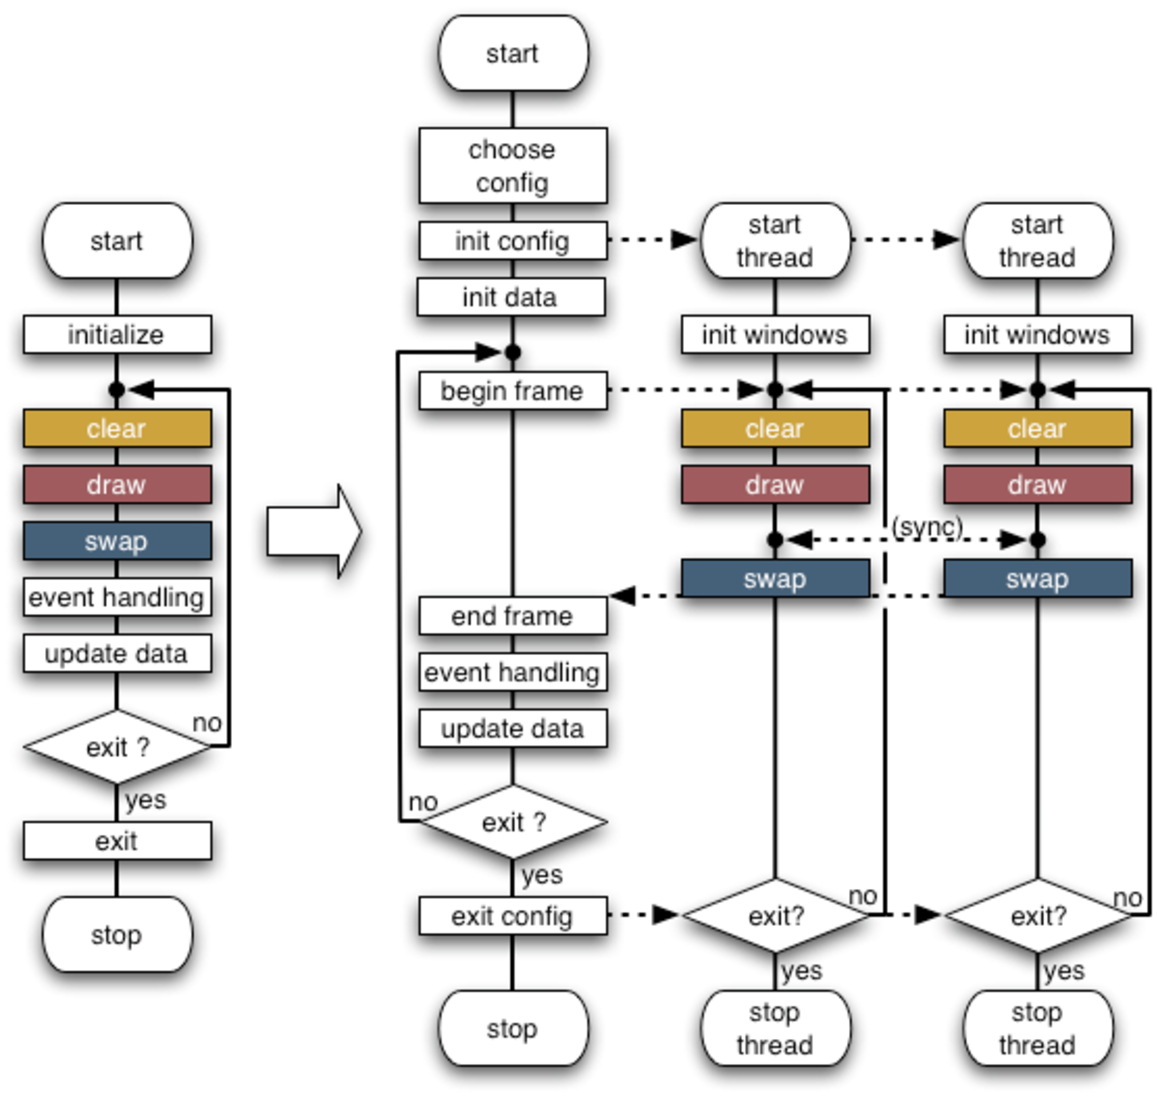
\includegraphics[scale=0.4]{../figures/parallel_rendering_execution_flow}
\caption{Paralleles Rendering (Quelle: [5])}
\end{center}
\end{figure}

\subsection{Equalizer}
Equalizer ist ein Framework zur Erstellung von parallelen, OpenGL-basierten Applikationen. Es erm"oglicht, Applikationen auf mehreren Grafikkarten, Prozessoren und Computern zu renderen und somit die Performance zu verbessern. 
Eine auf Equalizer basierende Applikation kann unver"andert aus verschiedenen Visualisierungssystemen ( Workstations, Cluster, Virtual Reality Installationen, etc) gestartet werden.

\paragraph{}
Das Equalizer-Projekt ist richtungsweisend und einzigartig was paralleles Rendering anbelangt. Initiator und Hauptentwickler Stefan Eilemann ist der BFH-TI nicht unbekannt und mit ihm wurden bereits Kontakte gekn"upft. Da es nichts vergleichbares gibt und gute Kontakte bestehen, ist die Verwendung von Equalizer vorgegeben. Ausserdem wird Equalizer rege genutzt und stetig weiterentwickelt. 

\subsubsection{Equalizer im CAVE}
Equalizer unterst"utzt sowohl aktives wie auch passives Stereo Rendering. Dabei gibt es die M"oglichkeit, dass jede Stereo View auf einer separaten CPU und Grafikkarte gerenderet werden kann. 

\begin{figure}[ht]
\begin{center}
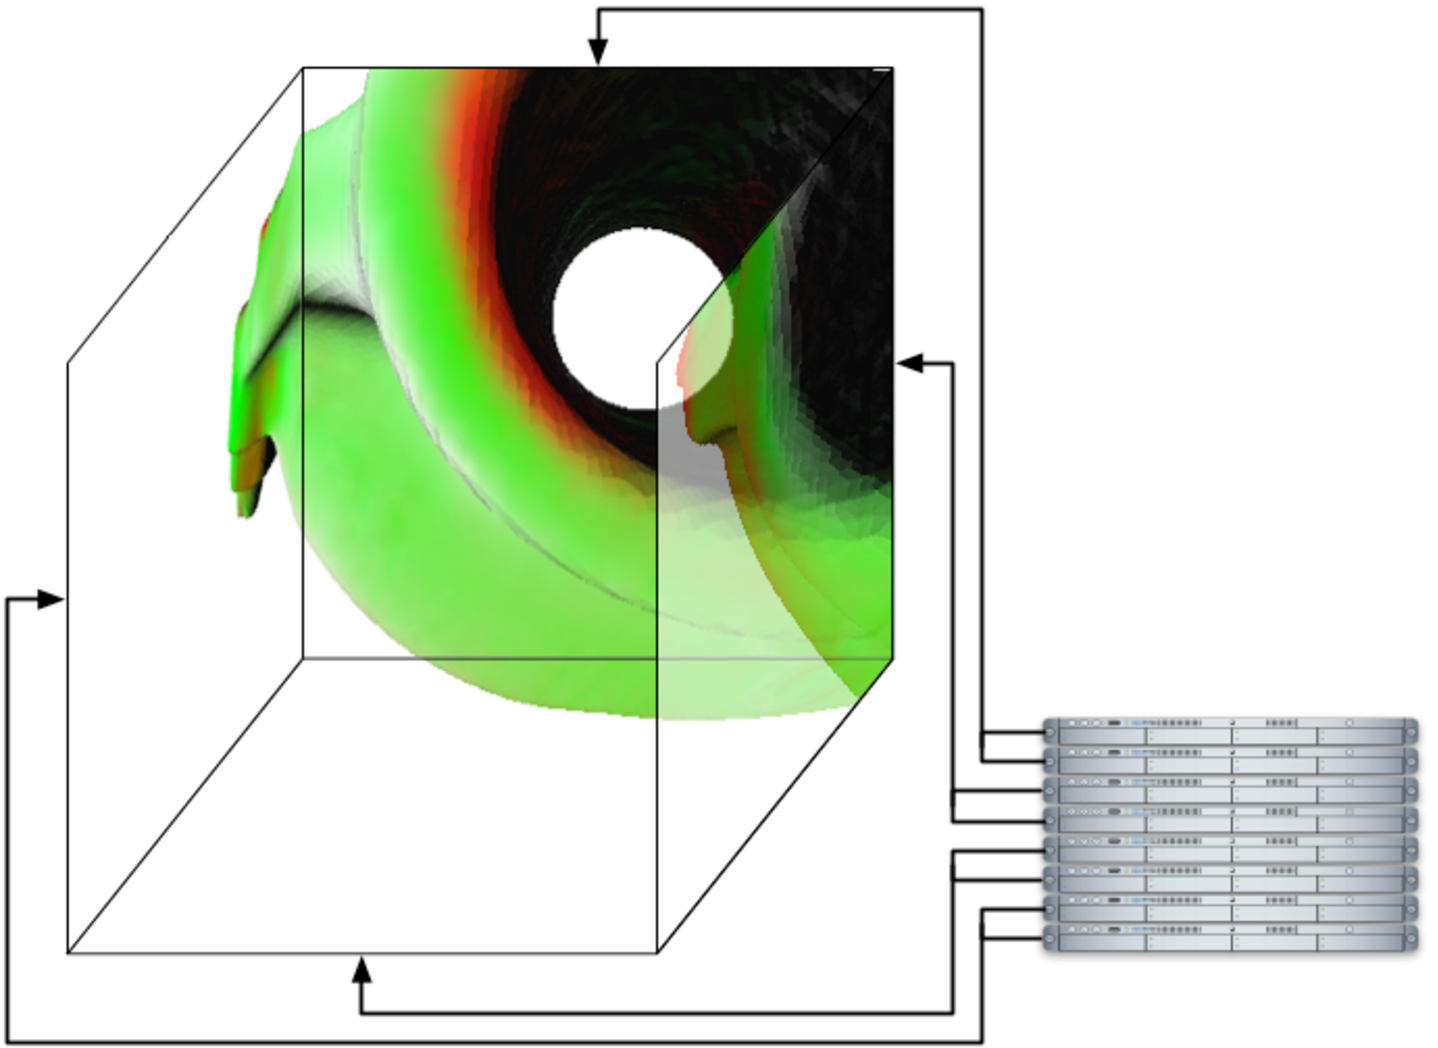
\includegraphics[scale=0.3]{../figures/equalizer_cave}
\end{center}
\caption{Equalizer im CAVE (Quelle: [5])}
\end{figure} 

\begin{figure}[ht]
\begin{center}
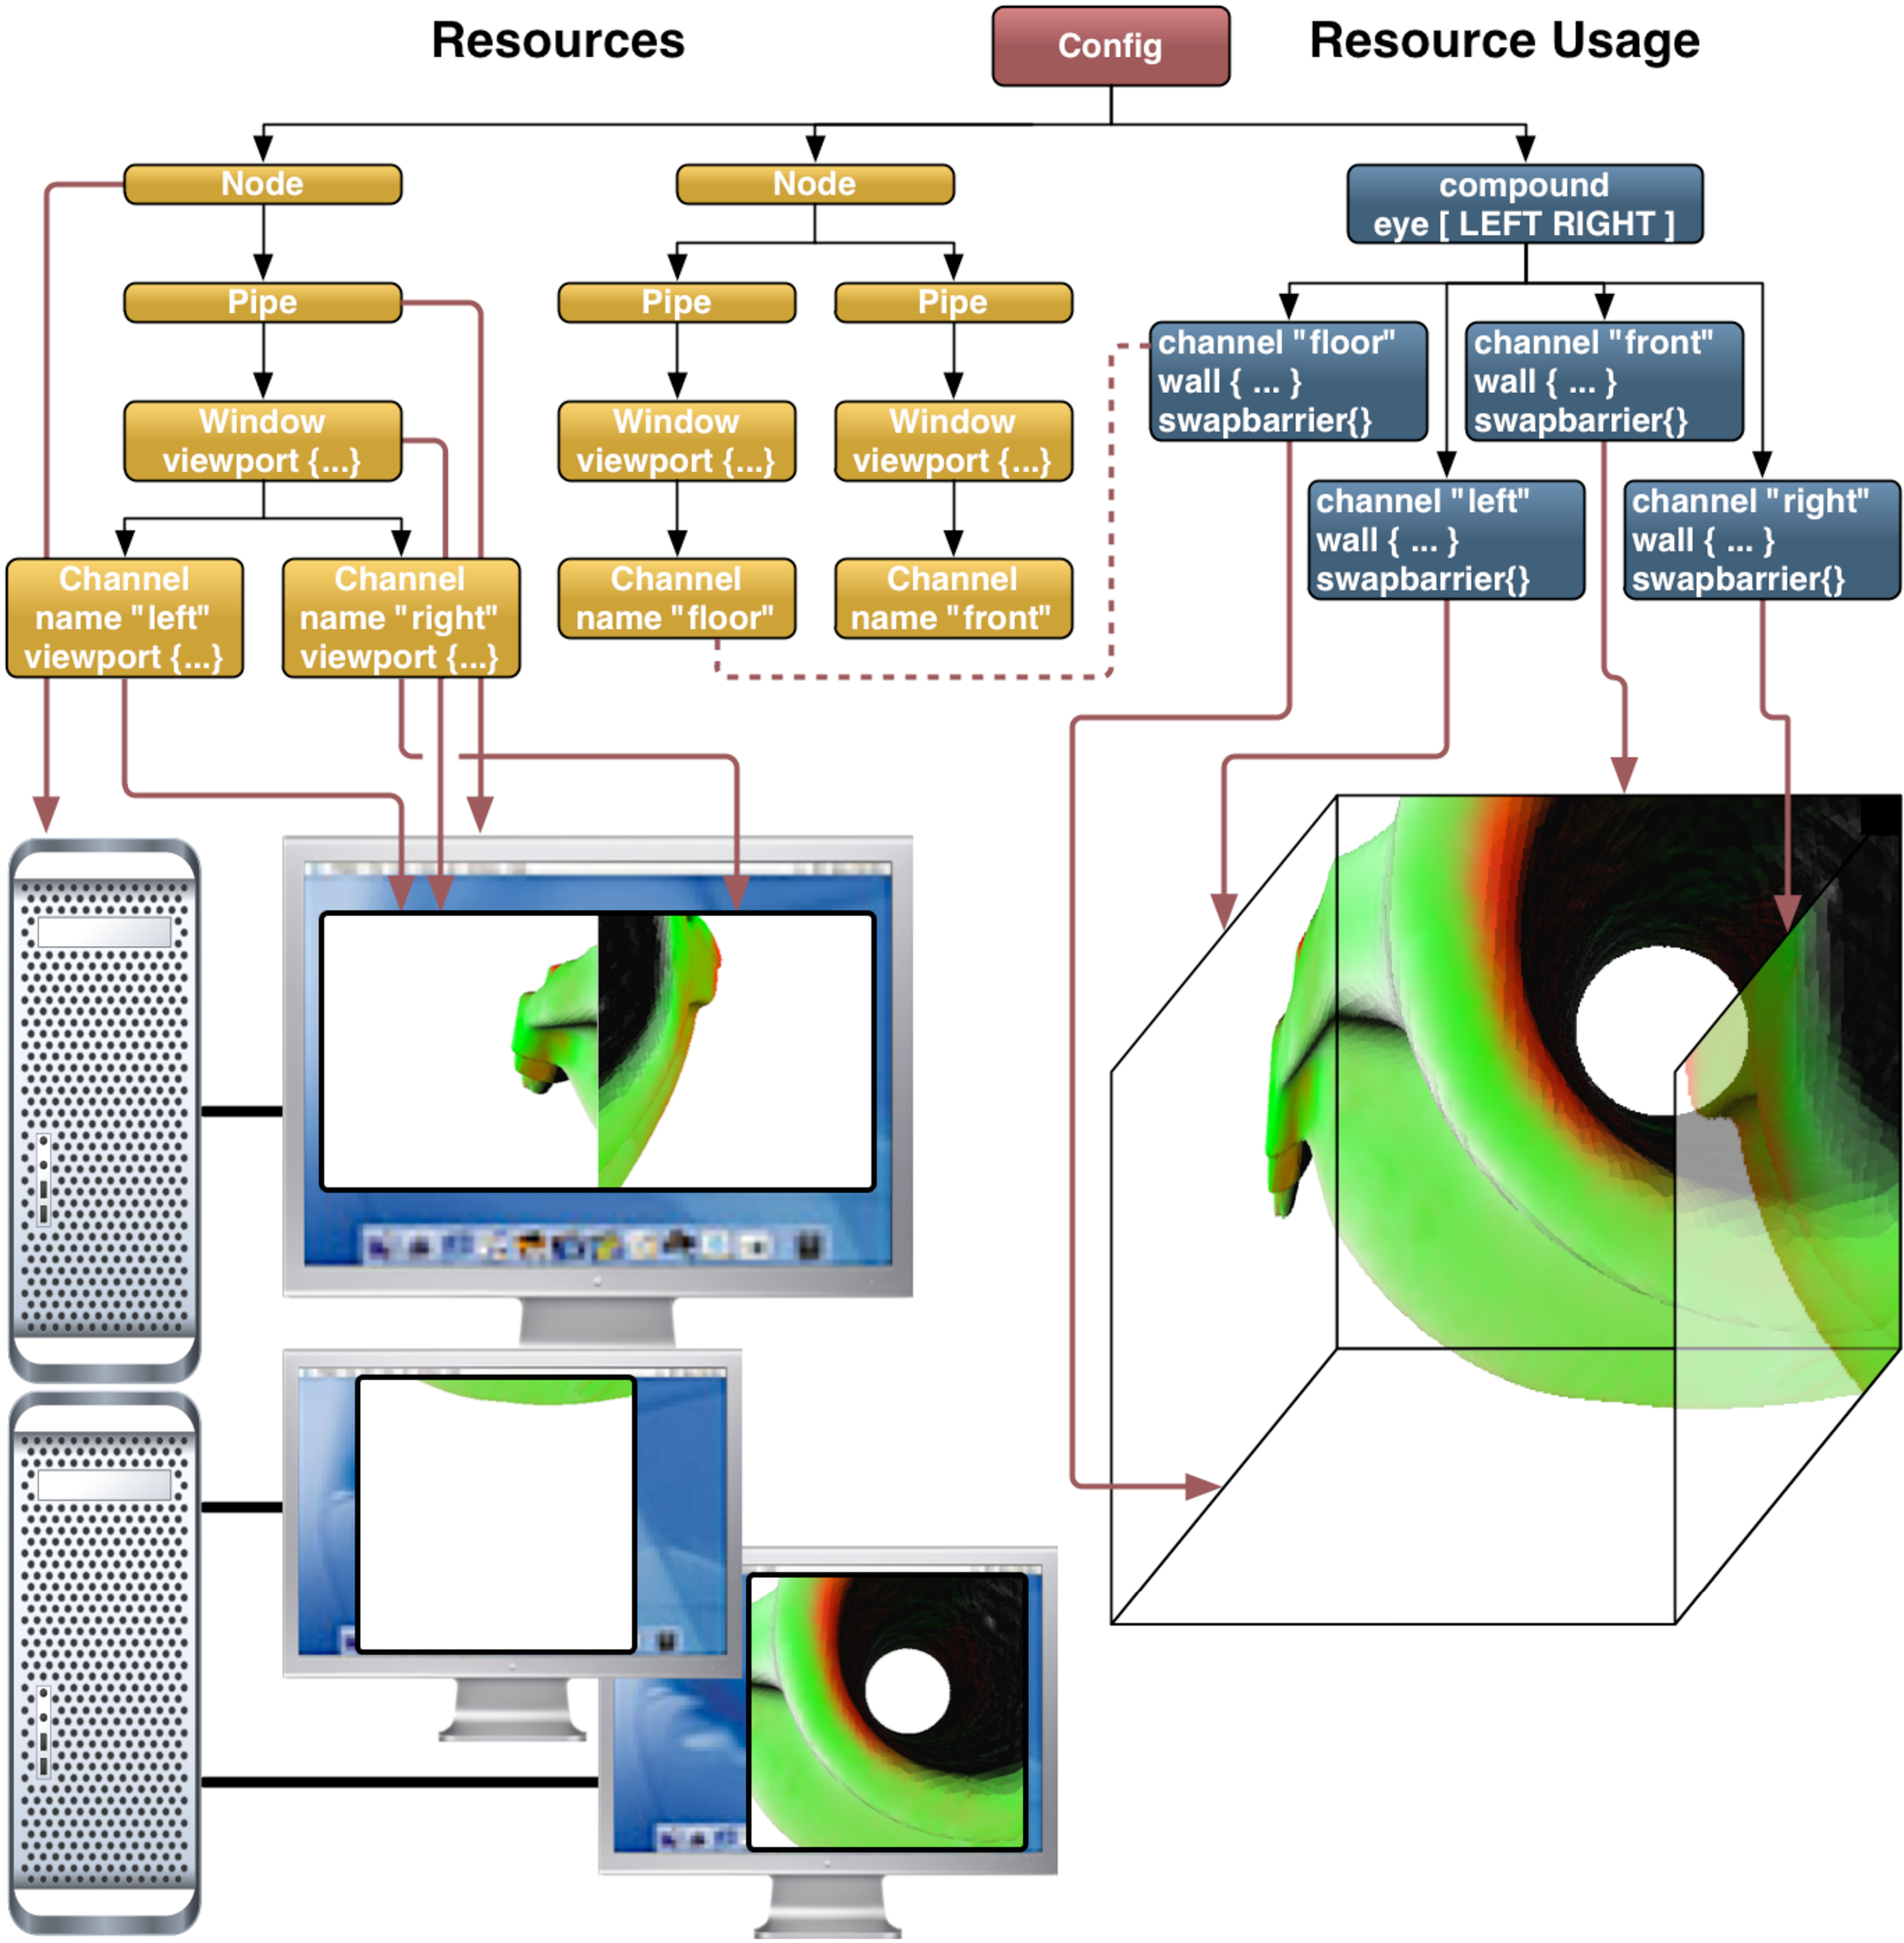
\includegraphics[scale=0.2]{../figures/equalizer_resources}
\end{center}
\caption{Equalizer im CAVE - Beispiel Konfiguration (Quelle: [1, Seite 10]}
\label{eq_ex_config}
\end{figure}

